\documentclass{article}
\usepackage[T1]{fontenc}
\usepackage{polski}
\usepackage[polish]{babel}
\usepackage[utf8x]{inputenc}
\usepackage{fontspec}
\usepackage{mathtools}
\usepackage{amssymb}
\usepackage[hidelinks]{hyperref}
\usepackage{amsmath,suetterl,graphicx,mathrsfs}
\usepackage{tabularx}
\usepackage[a4paper, total={6.2in, 10in}]{geometry}
\usepackage[skip=4pt plus1pt, indent=0pt]{parskip}

\title{SIK zadanie 3}
\author{Bartosz Kucypera}
\date{\today}

\begin{document}

\maketitle

\section*{Logiczne połączenie ruterów}
Załóżmy, że serwery dns są w sieci razem z R12. \newline
Załóżmy, że pierwsza sieć przez którą idą pakiety z R13 do eagle-a to 208.42.42.0/24. \newline
Załóżmy, że pierwsza sieć przez którą idą pakiety z R14 do kestrel-a to 209.42.42.0/24. \newline

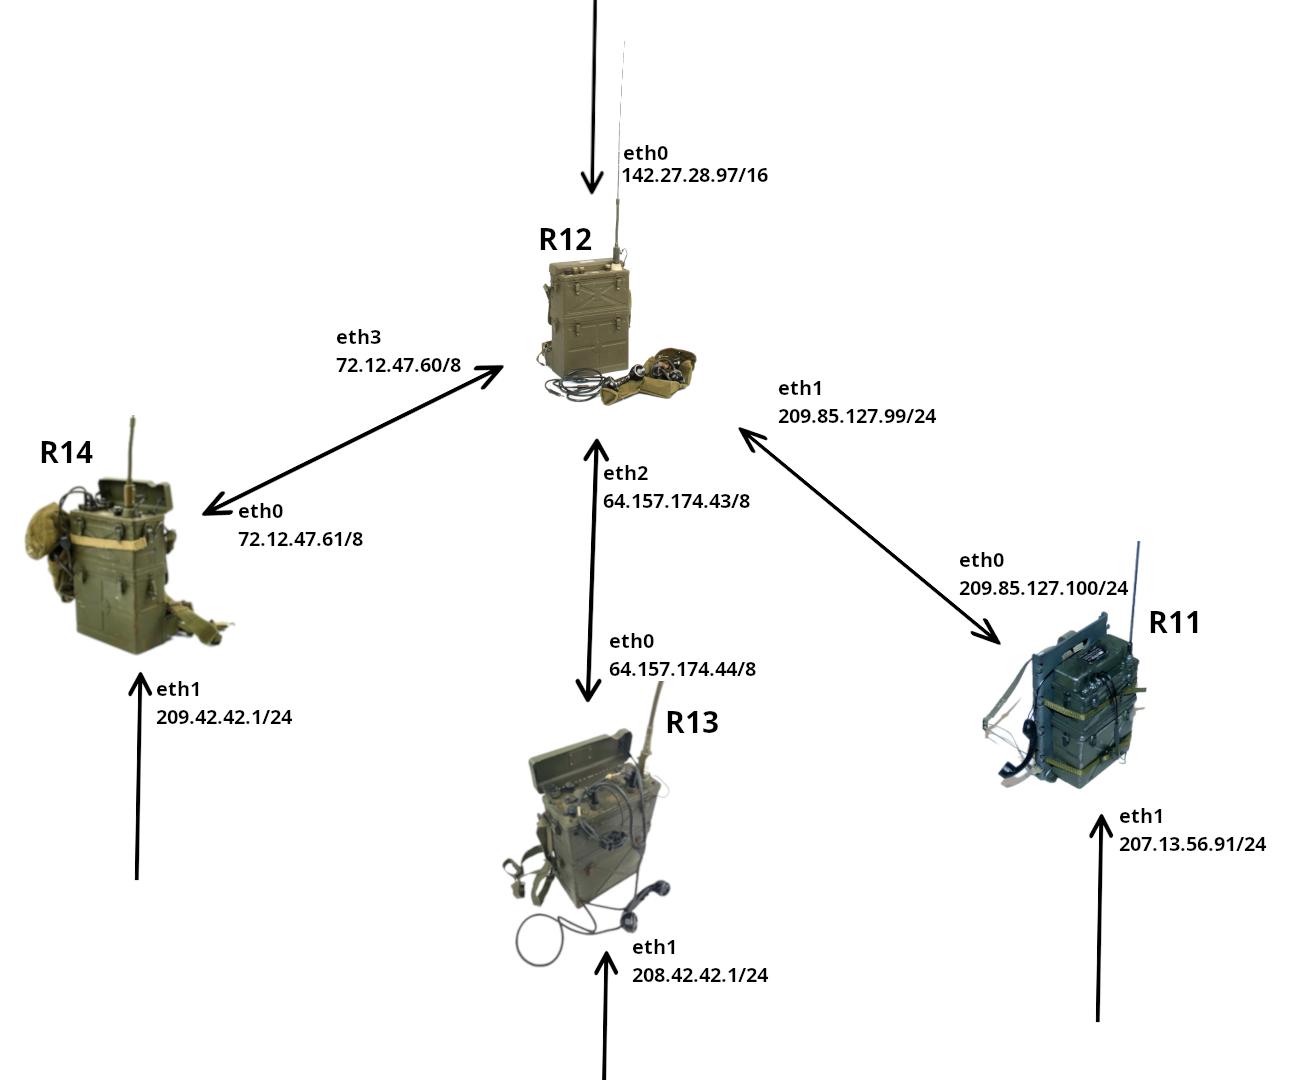
\includegraphics[width=\linewidth]{sieci.png}
\newpage

\section*{Fragment tablicy tras rutera R12}
\begin{tabularx}{0.8\textwidth} { 
  | >{\raggedright\arraybackslash}X 
  | >{\centering\arraybackslash}X 
  | >{\centering\arraybackslash}X
  | >{\raggedleft\arraybackslash}X| }
  	\hline
	adres & maska & interfejs & brama \\
	\hline
 	142.27.0.0 & 255.255.0.0 & eth0 & 0.0.0.0 \\
	\hline
 	209.85.127.0 & 255.255.255.0 & eth1 & 0.0.0.0 \\
	\hline
	222.67.1.0 & 255.255.255.0 & eth1 & 209.85.127.100 \\
 	\hline
	64.0.0.0 & 255.0.0.0 & eth2 & 0.0.0.0 \\
	\hline
	25.0.0.0 & 255.0.0.0 & eth2 & 64.157.174.44 \\
	\hline
	72.0.0.0 & 255.0.0.0 & eth3 & 0.0.0.0 \\
	\hline
	193.19.88.0 & 255.255.255.0 & eth3 & 72.12.47.61 \\
\hline
\end{tabularx}

\section*{Wynik traceroute z eagle-a do pigeon-a}
traceroute to pigeon.zad3sik.edu.pl (222.67.1.27), 30 hops max, 60 byte packets \newline
 1 * * * \newline
 2 * * * \newline
 3 R13.zad3sik.edu.pl (208.42.42.1) \newline
 4 R12.zad3sik.edu.pl (64.157.174.43) \newline
 5 R11.zad3sik.edu.pl (209.85.127.100) \newline
 6 * * * \newline
 7 * * * \newline
 8 * * * \newline
9 * * * \newline
10 * * * \newline
11 * * * \newline
12 * * * \newline
13 pigeon.zad3sik.edu.pl (222.67.1.27) \newline

\section*{Wynik traceroute z kestrel-a do pigeon-a}
traceroute to pigeon.zad3sik.edu.pl (222.67.1.27), 30 hops max, 60 byte packets \newline
 1 * * * \newline
 2 * * * \newline
 3 * * * \newline
 4 * * * \newline
 5 * * * \newline
 6 R14.zad3sik.edu.pl (209.42.42.1) \newline
 7 R12.zad3sik.edu.pl (72.12.47.60) \newline
 8 R11.zad3sik.edu.pl (209.85.127.100) \newline 
 9 * * * \newline
10 * * * \newline
11 * * * \newline
12 * * * \newline
13 * * * \newline
14 * * * \newline
15 * * * \newline
16 pigeon.zad3sik.edu.pl (222.67.1.27) \newline

\newpage
\section*{Plik zad3.sik.edu.pl}
\$ TTL 1h
@ IN SOA ns.zad3sik.edu.pl. bk439964.zad3sik.edu.pl. ( \\
\hspace*{3cm}1 ; Serial \\
\hspace*{3cm}604800 ; Refresh \\
\hspace*{3cm}86400 ; Retry \\
\hspace*{3cm}2419200 ; Expire\\
\hspace*{3cm}604800) ; Negative Cache TTL\\

@ \hspace{4cm} IN NS ns1.zad3sik.edu.pl. \\
@ \hspace{4cm} IN NS ns2.zad3sik.edu.pl. \\
\\
ns1 \hspace{3.8cm} IN A 142.27.28.98\\
ns2 \hspace{3.8cm} IN A 142.27.28.99 \\
R11 \hspace{3.7cm} IN A 209.85.10.100 \\
R11 \hspace{3.7cm} IN A 207.13.56.91 \\
R12 \hspace{3.7cm} IN A 142.27.28.97 \\
R12 \hspace{3.7cm} IN A 209.85.127.99 \\
R12 \hspace{3.7cm} IN A 64.157.174.43 \\
R12 \hspace{3.7cm} IN A 72.12.47.60 \\
R13 \hspace{3.7cm} IN A 64.157.174.44 \\
R13 \hspace{3.7cm} IN A 208.42.42.1 \\
R14 \hspace{3.7cm} IN A 72.12.47.61 \\
R14 \hspace{3.7cm} IN A 209.42.42.1 \\
pigeon \hspace{3.3cm} IN A 222.67.1.27 \\
eagle \hspace{3.55cm} IN A 25.3.143.12 \\
kestrel \hspace{3.3cm} IN A 193.19.88.91 \\




\end{document}
